\section{Benchmark}\label{sec:benchmark}

In this section, we study a wide array of benchmarks.

\subsection{Block Update Comparison}\label{ssec:benchmark:pgd-newton}

In this section, we compare the algorithms presented 
in~\Cref{ssec:pgd,ssec:newton,ssec:newton-abs}
that solve the block update~(\ref{eq:bcd:block-update}).
Recall the objective to solve is
\begin{align*}
    \minimize_{\beta \in \R^p}
    \frac{1}{2} \beta^\top \Sigma \beta
    - v^\top \beta
    + \lambda \norm{\beta}_2
\end{align*}

\Cref{fig:bench:newton-compare} shows a set of comparisons
Newton, Brent, and Newton-ABS
(see~\Cref{ssec:newton,ssec:newton-abs}).
Although we also ran ISTA, FISTA, and FISTA with adaptive restart (FISTA-ADA)
(see~\Cref{ssec:pgd}), they failed to converge, so we omit their benchmark results.
All Newton methods properly converged.
For all scenarios, the diagonal of $\Sigma$ was generated uniformly from $[0, 1]$.
In addition,
\begin{enumerate}
    \item[(b)] \textbf{Almost PSD:} 1\% of the entries were regenerated uniformly from $[\num{1e-14}, \num{1e-8}]$.
    \item[(c)] \textbf{Very PSD:} 20\% of the entries were set exactly to zero and 10\% were regenerated from $[\num{1e-14}, \num{1e-8}]$.
\end{enumerate}
The vector $v$ was generated from $\Normal\pr{0, \Sigma}$.
Figures (a) to (c) used $\lambda=\num{1e-1}$ while (d) used $\lambda=\num{1e-4}$.
Both Newton-ABS and Brent methods are asymptotically faster than Newton,
however, Brent has the poorest performance for small to moderate $p$ ($\leq 100$).
Although, Brent performs slightly better than Newton-ABS when $D$ is positive definite,
we see that Newton-ABS is faster than Brent uniformly over $p$ when $D$ is PSD
by a larger margin.
Newton-ABS is up to 7 times faster than Newton and up to 4 times faster than Brent.
Given the robustness of Newton-ABS in speed and convergence across the different configurations,
we expect significant improvement to the overall optimizer using Newton-ABS.

\begin{figure}[t]
    \centering 
    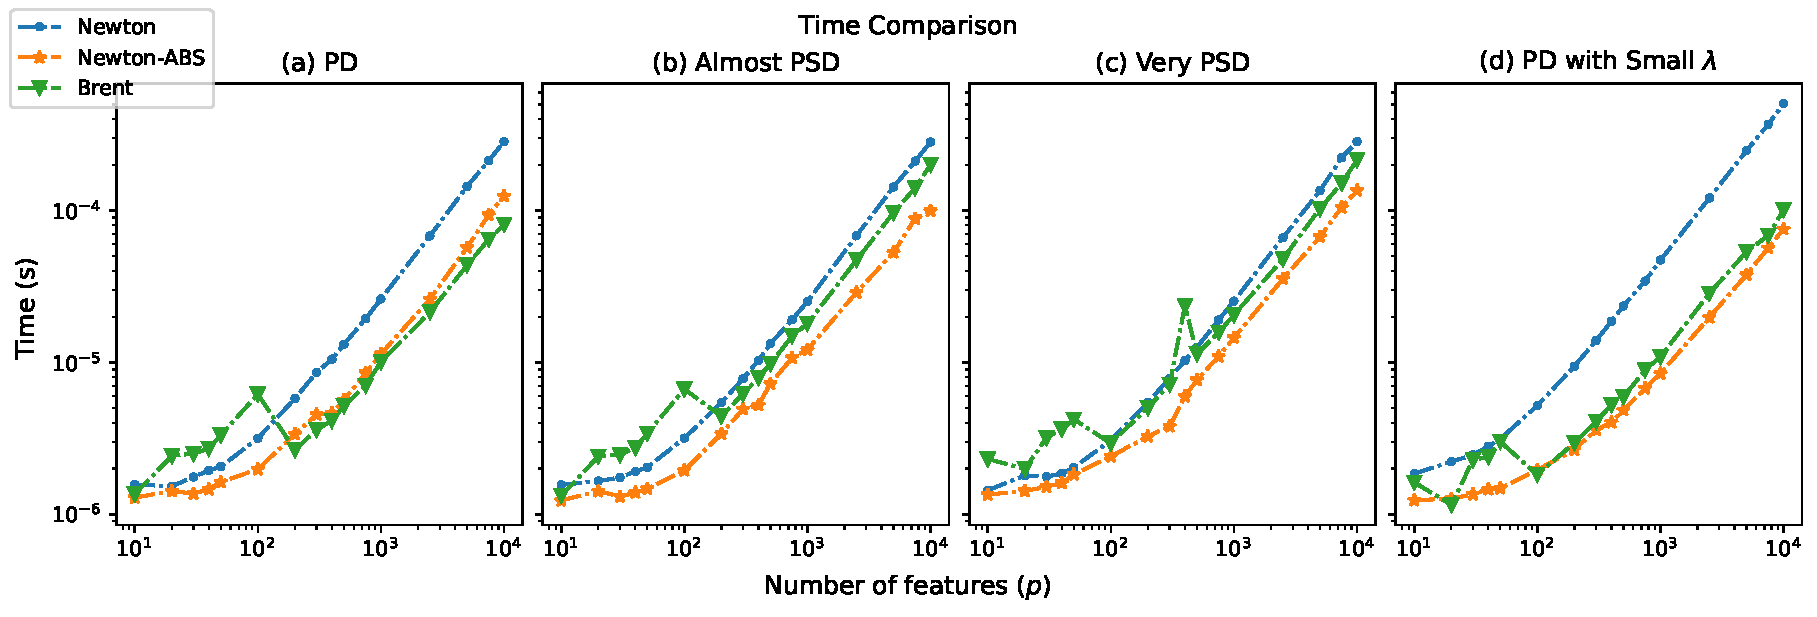
\includegraphics[width=\textwidth]{figures/newton_compare.pdf}
    \caption{Plot of runtimes for Newton, Newton-ABS, and Brent's Method
    for various input configurations.
    Figures (a) to (c) modifies the singularity of $D$ from positive definite to positive semi-definite.
    Figure (d) changes the regularization level to a smaller value.
    Overall, Newton-ABS is generally faster than Newton and Brent.
    Newton-ABS is up to 7 times faster than Newton and up to 4 times faster than Brent.
    }
    \label{fig:bench:newton-compare}
\end{figure}

%\begin{figure}[t]
%    \centering
%    \begin{subfigure}[b]{0.49\textwidth}
%        \centering
%        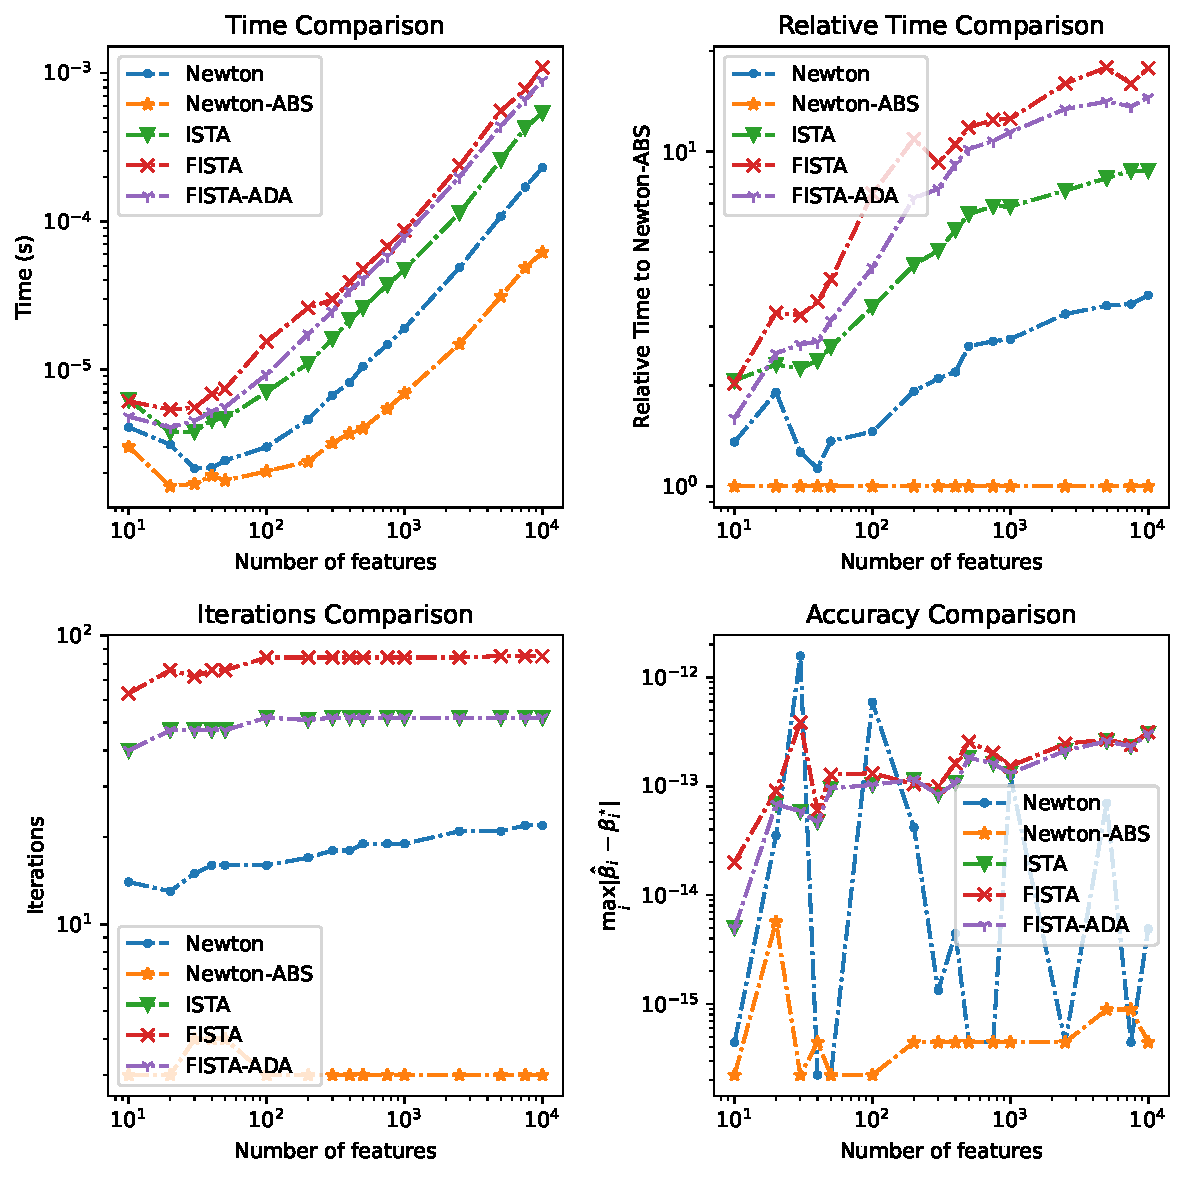
\includegraphics[width=\textwidth]{figures/pgd_newton_pd.pdf}
%        \caption{Positive definite}
%        \label{fig:bench:pgd-newton:pd}
%    \end{subfigure} 
%    \hfill
%    \begin{subfigure}[b]{0.49\textwidth}
%        \centering
%        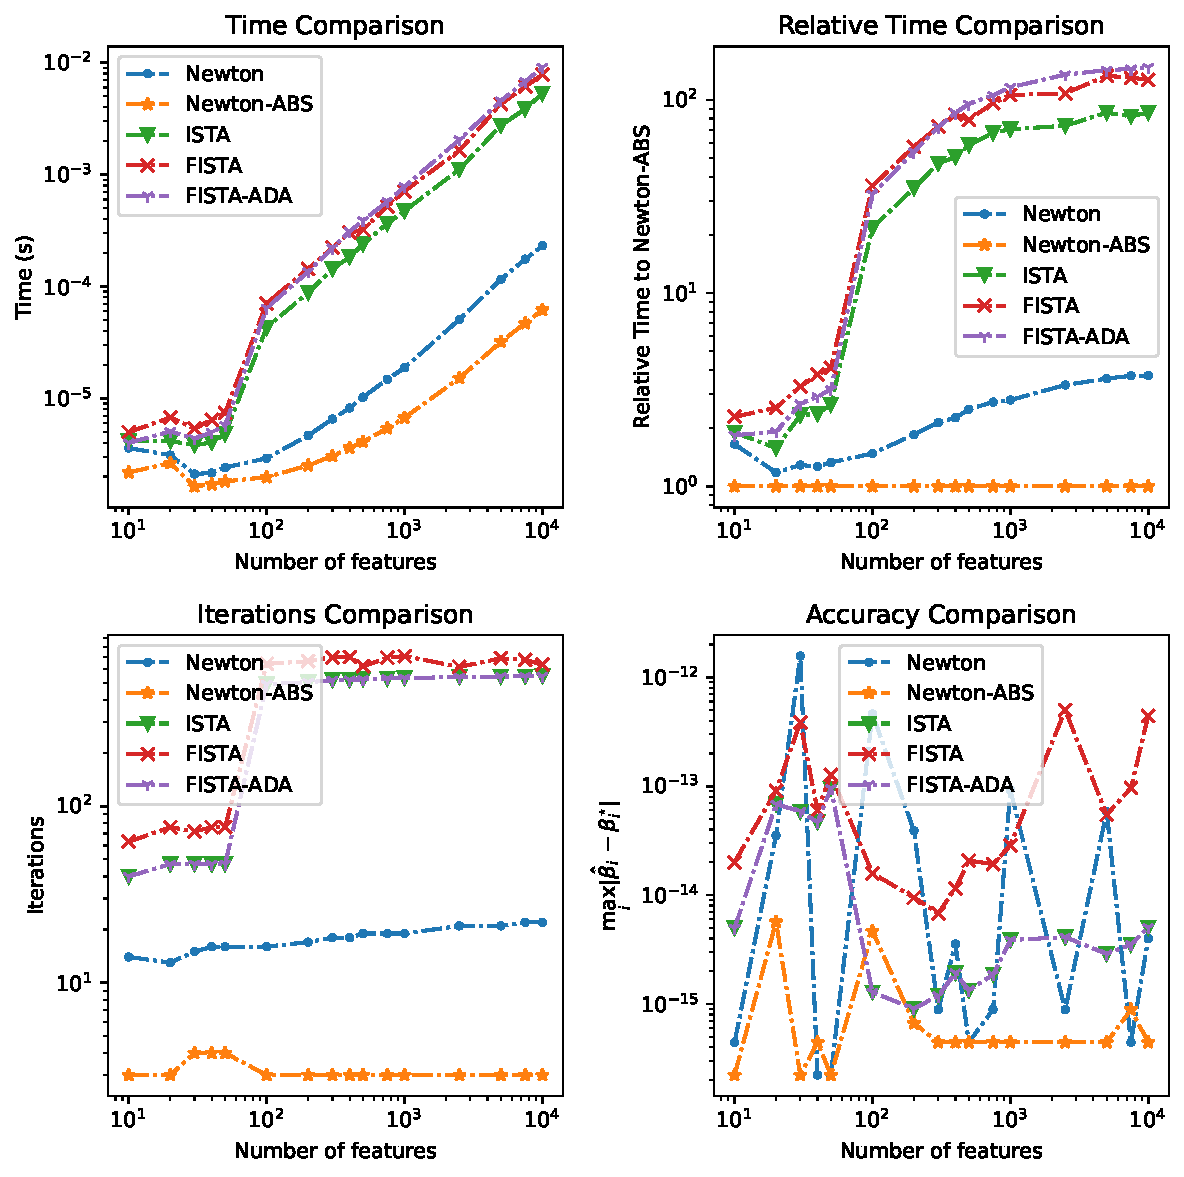
\includegraphics[width=\textwidth]{figures/pgd_newton_almost_psd.pdf}
%        \caption{Almost semi-definite}
%        \label{fig:bench:pgd-newton:almost_psd}
%    \end{subfigure} 
%    \\
%    \begin{subfigure}[b]{0.49\textwidth}
%        \centering
%        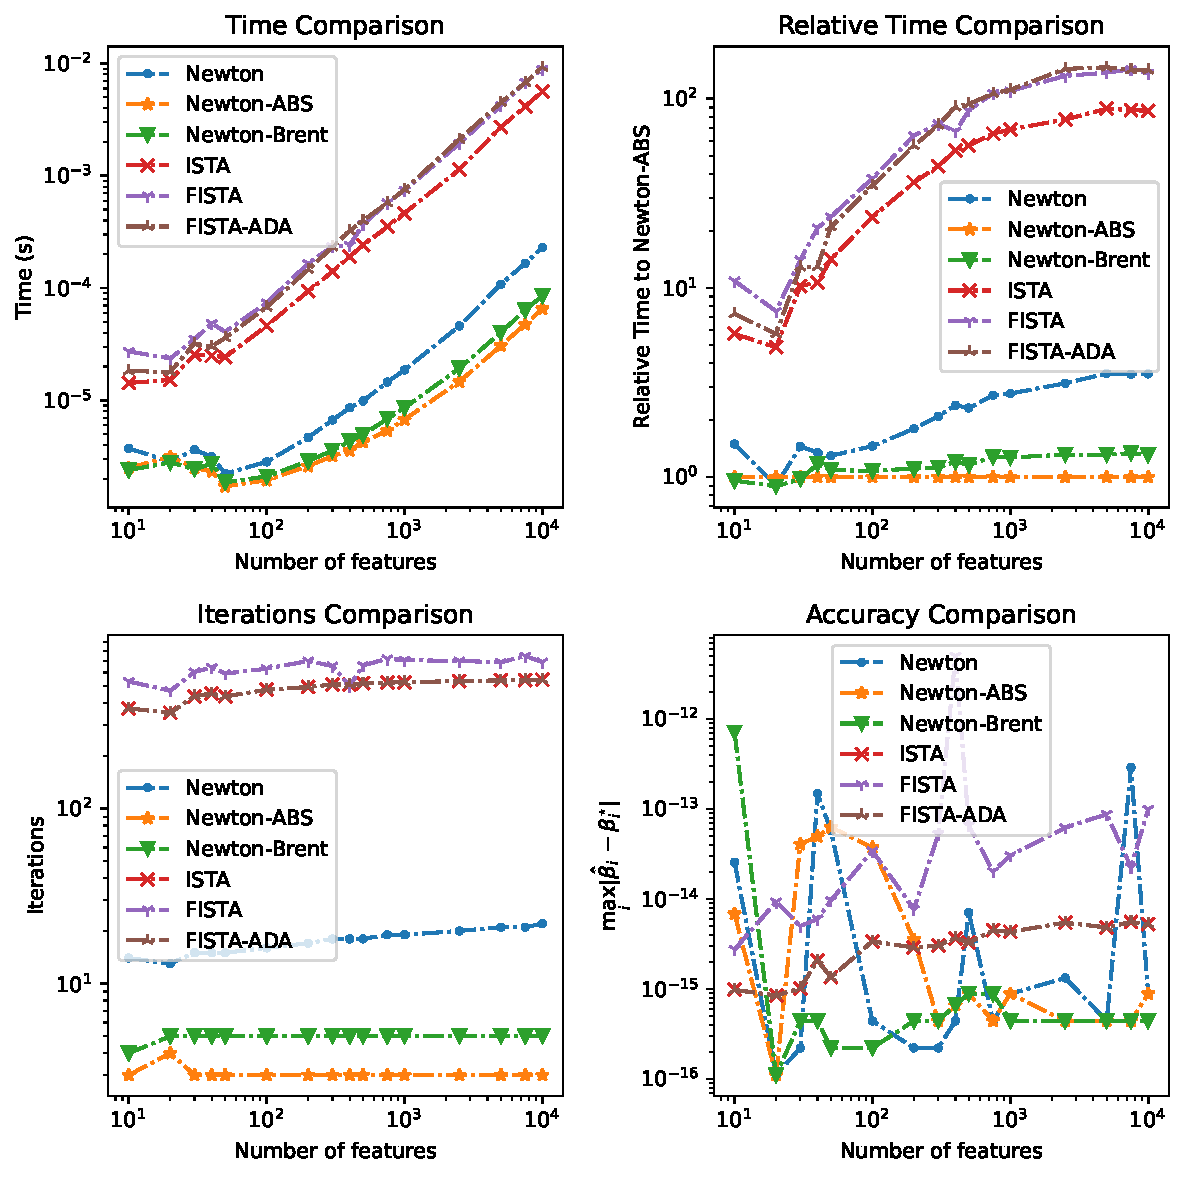
\includegraphics[width=\textwidth]{figures/pgd_newton_very_psd.pdf}
%        \caption{Very semi-definite}
%        \label{fig:bench:pgd-newton:very_psd}
%    \end{subfigure} 
%    \hfill
%    \begin{subfigure}[b]{0.49\textwidth}
%        \centering
%        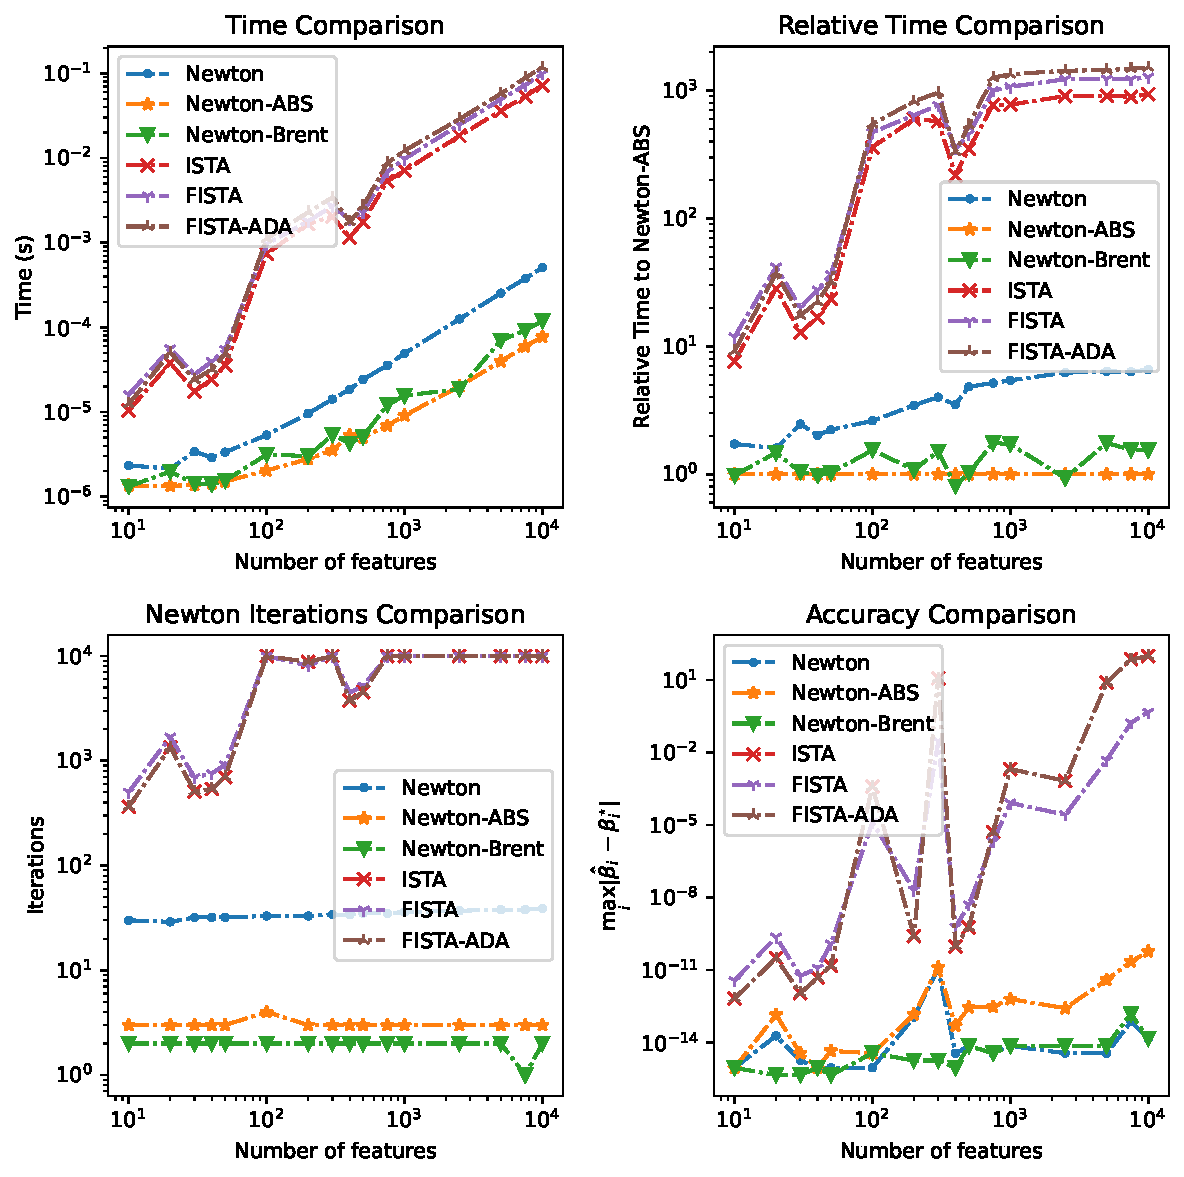
\includegraphics[width=\textwidth]{figures/pgd_newton_low_regul.pdf}
%        \caption{Positive definite and low regularization}
%        \label{fig:bench:pgd-newton:low_regul}
%    \end{subfigure} 
%    \caption{%
%        \Cref{%
%            fig:bench:pgd-newton:low_regul,%
%            fig:bench:pgd-newton:almost_psd,%
%            fig:bench:pgd-newton:pd,%
%            fig:bench:pgd-newton:very_psd%
%        }
%        show a comparison of time, relative time, number of iterations, and accuracy
%        across different algorithms.
%        \Cref{%
%            fig:bench:pgd-newton:almost_psd,%
%            fig:bench:pgd-newton:pd,%
%            fig:bench:pgd-newton:very_psd%
%        } fixed $\lambda=\num{1e-1}$ while 
%        \Cref{fig:bench:pgd-newton:pd} fixed $\lambda=\num{1e-4}$.
%        The difference across
%        \Cref{%
%            fig:bench:pgd-newton:almost_psd,%
%            fig:bench:pgd-newton:pd,%
%            fig:bench:pgd-newton:very_psd%
%        } is the degree of singularity of $D$.
%        \Cref{fig:bench:pgd-newton:pd} used a positive definite $D$,
%        \Cref{fig:bench:pgd-newton:almost_psd} used a positive definite $D$ with
%        some eigenvalues close to $0$ (but not exactly), and
%        \Cref{fig:bench:pgd-newton:very_psd} used a positive semi-definite $D$
%        with some eigenvalues exactly at $0$, some close to $0$, and some sufficiently positive.
%        Overall, the Newton methods clearly outshine the PGD methods in terms of speed
%        with Newton-ABS in the obvious lead.
%    }
%    \label{fig:bench:pgd-newton}
%\end{figure}
